\chapter{Modèle ALM interne et construction de la base de données}

Ce chapitre présente le modèle ALM utilisé dans le cadre de ce mémoire ainsi que la méthodologie mise en place pour construire la base de données. Dans un premier temps, le fonctionnement général du modèle SALLTO est décrit. Dans un second temps, le portefeuille étudié et les différentes sensibilités réalisées sont présentés. Enfin, la méthode de construction de la base de données et l'automatisation des lancements sont détaillées.


% =============================================================================
% MODÈLE ALM
% =============================================================================

\section{Le modèle ALM interne}

Au sein de Forsides, le modèle ALM utilisé s'appelle SALLTO (\textit{Solvency Asset Liability Life TOols}). Il s'agit d'un outil développé et codé en interne en C\#. Ce modèle permet de représenter l'évolution dans le temps d'une compagnie d'assurance vie, en intégrant explicitement les interactions entre l'actif et le passif à partir de scénarios économiques.

L'objectif d'un modèle ALM est de projeter conjointement les actifs détenus par l'assureur et les engagements envers les assurés. Cette projection permet notamment de prendre en compte les interactions entre les conditions économiques, les caractéristiques du portefeuille, les comportements des assurés et la politique de gestion de la compagnie.

Pour fonctionner, SALLTO nécessite un fichier d'entrée dans lequel sont renseignées différentes hypothèses. Ces hypothèses concernent :

\begin{itemize}
    \item les caractéristiques de l'actif ;
    \item les caractéristiques du passif ;
    \item les hypothèses de comportement des assurés ;
    \item les tables de mortalité ;
    \item la politique de gestion de la compagnie ;
    \item les scénarios économiques utilisés pour les projections.
\end{itemize}

Les scénarios économiques sont générés indépendamment par un générateur de scénarios économiques, appelé GSE. Ils sont ensuite intégrés dans le fichier d'entrée de SALLTO et servent de base aux différentes projections réalisées par le modèle.

La Figure~\ref{fig:schema_sallto} présente de manière synthétique le fonctionnement général de SALLTO et les différentes données nécessaires à son utilisation.

\begin{figure}[H]
    \centering
    \includegraphics[width=0.9\textwidth]
    {images/2_chapitres/chapitre2/Schema_SALLTO.png}
    \caption{Schéma général de fonctionnement de SALLTO}
    \label{fig:schema_sallto}
\end{figure}


\subsection{Le générateur de scénarios économiques}

Le générateur de scénarios économiques permet de produire un ensemble de trajectoires possibles pour les principales variables économiques et financières utilisées dans le modèle. Ces trajectoires concernent notamment les taux d'intérêt, les actions et l'immobilier.

Le GSE est calibré à partir de données issues des marchés financiers. Il génère ensuite plusieurs scénarios représentant différentes évolutions possibles de l'environnement économique sur l'horizon de projection.

Ces scénarios sont utilisés dans les calculs stochastiques de SALLTO. Pour chaque scénario économique, le modèle projette l'évolution de l'actif, du passif et des décisions de gestion. La moyenne des résultats obtenus sur l'ensemble des scénarios permet ensuite de déterminer le Best Estimate stochastique.

Dans le cadre de cette étude, plusieurs paramétrages du GSE sont utilisés afin de faire varier la courbe des taux, la volatilité des taux et la volatilité des actions.


\subsection{Fonctionnement de SALLTO}

À partir du fichier d'entrée, des scénarios économiques et des tables de mortalité, SALLTO projette l'évolution du portefeuille sur l'ensemble de l'horizon retenu.

Pour chaque pas de temps et pour chaque scénario économique, le modèle simule notamment :

\begin{itemize}
    \item l'évolution de la valeur des actifs ;
    \item les produits financiers générés par le portefeuille ;
    \item les prestations versées aux assurés ;
    \item les rachats ;
    \item la participation aux bénéfices ;
    \item les décisions de gestion prises par l'assureur ;
    \item l'évolution des provisions mathématiques.
\end{itemize}

Les interactions entre l'actif et le passif sont prises en compte au cours de chaque projection. Par exemple, le rendement des actifs influence la capacité de l'assureur à revaloriser les contrats. En retour, le niveau de revalorisation peut modifier le comportement de rachat des assurés et donc les flux futurs du passif.

À l'issue des projections, SALLTO produit un fichier de résultats contenant notamment les flux de trésorerie, les résultats nécessaires aux calculs Solvabilité~II ainsi que les différents éléments de valorisation du portefeuille.

Dans le cadre de ce mémoire, les principaux résultats utilisés sont :

\begin{itemize}
    \item le Best Estimate déterministe ;
    \item le Best Estimate stochastique ;
    \item l'écart entre ces deux valorisations.
\end{itemize}


% =============================================================================
% PORTEFEUILLE
% =============================================================================

\section{Description du portefeuille étudié}


La construction de la base de données nécessaire à l'étude repose sur la définition préalable d'un portefeuille central, à partir duquel seront réalisées les différentes sensibilités présentées par la suite.

Le portefeuille retenu est un portefeuille fictif, valorisé au 31 décembre 2025. Il a été construit à partir de données de marché et d'hypothèses représentatives des caractéristiques généralement observées au sein des portefeuilles d'assureurs vie. L'objectif n'est donc pas de reproduire le bilan d'un assureur particulier, mais de disposer d'un portefeuille de référence cohérent avec les pratiques du marché et suffisamment représentatif pour les besoins de l'étude.

Ce portefeuille constitue le point de départ de l'ensemble des projections réalisées dans la suite du mémoire. Les résultats obtenus, et en particulier la relation mise en évidence entre le Best Estimate déterministe et le Best Estimate stochastique, restent ainsi conditionnés aux caractéristiques du portefeuille central retenu. Cette dépendance devra être prise en compte dans l'interprétation des résultats.

\subsection{Portefeuille d'actifs}

Le portefeuille d'actifs présenté dans cette section correspond aux actifs en représentation du fonds euro. Sa valeur nette comptable totale s'élève à 116 millions d'euros au 31 décembre 2025, tandis que sa valeur de marché atteint 113,39 millions d'euros.

L'allocation a été définie de manière à reproduire la structure d'un portefeuille d'actifs représentatif d'un assureur vie. En valeur nette comptable, elle se compose de 80\,\% d'obligations à taux fixe, 10\,\% d'actions globales non long terme, 7\,\% d'immobilier et 3\,\% d'actifs monétaires.

\begin{table}[H]
    \centering
    \caption{Allocation du portefeuille d'actifs central}
    \label{tab:allocation_actif_central}
    \begin{tabular}{lcc}
        \hline
        \textbf{Classe d'actifs} & \textbf{Allocation en VNC} & \textbf{PMVL} \\
        \hline
        Monétaire & 3\,\% & 0\,\% \\
        Actions globales non long terme & 10\,\% & +30\,\% \\
        Immobilier & 7\,\% & +10\,\% \\
        Obligations à taux fixe & 80\,\% & -7\,\% \\
        \hline
        \textbf{Total} & \textbf{100\,\%} & \textbf{$\approx -2\,\%$} \\
        \hline
    \end{tabular}
\end{table}

Les différentes classes d'actifs présentent des niveaux de plus ou moins-values latentes distincts. Les actions présentent ainsi une plus-value latente de 30\,\% et l'immobilier de 10\,\%, tandis que la poche obligataire présente une moins-value latente de 7\,\%. Compte tenu du poids prépondérant des obligations dans l'allocation, le portefeuille présente globalement une légère moins-value latente, de l'ordre de 2\,\%.

La poche obligataire représente 80\,\% de la VNC totale du portefeuille d'actifs et constitue ainsi sa principale composante. Elle est composée à 60\,\% d'obligations souveraines et à 40\,\% d'obligations corporate. Le portefeuille obligataire présente un rating moyen de A.

Le spread moyen du portefeuille central est de 0,85\,\%, tandis que la duration moyenne de l'actif s'établit à 6,75. Ces caractéristiques permettent de définir l'exposition initiale du portefeuille aux principaux facteurs de risque de marché, avant application des différentes sensibilités considérées dans la suite de l'étude.

\begin{table}[H]
    \centering
    \caption{Principales caractéristiques du portefeuille d'actifs central}
    \label{tab:caracteristiques_actif_central}
    \begin{tabular}{lc}
        \hline
        \textbf{Caractéristique} & \textbf{Valeur} \\
        \hline
        Valeur nette comptable & 116 M\euro \\
        Valeur de marché & 113,39 M\euro \\
        Part d'obligations souveraines & 60\,\% de la poche obligataire \\
        Part d'obligations corporate & 40\,\% de la poche obligataire \\
        Rating obligataire moyen & A \\
        Spread moyen & 0,85\,\% \\
        Duration moyenne de l'actif & 6,75 \\
        Plus-value latente globale & $\approx -2\,\%$ \\
        \hline
    \end{tabular}
\end{table}


\subsection{Portefeuille de passifs}

Le portefeuille de passifs a également été construit afin de reproduire les principales caractéristiques d'un portefeuille moyen d'assurance vie. Il est constitué d'un encours total de provisions mathématiques (PM) de 145 millions d'euros, réparti entre 100 millions d'euros de PM euro et 45 millions d'euros de PM en unités de compte (UC). Les supports euro représentent ainsi environ 69\,\% des PM totales, contre 31\,\% pour les UC.

Afin de limiter les temps de calcul liés aux projections stochastiques, une hypothèse simplificatrice a été retenue concernant la segmentation du portefeuille. Le passif est représenté par seulement 10 model points, dont 5 associés au fonds euro et 5 aux UC. Cette réduction du nombre de model points permet d'alléger significativement les calculs tout en conservant une segmentation du portefeuille adaptée aux objectifs de l'étude.

L'âge moyen des assurés du portefeuille central est de 63 ans. Les frais de gestion sur encours sont fixés à 0,40\,\% et le taux de chargement à 0,80\,\%. Ces hypothèses sont identiques pour l'ensemble des model points.

Le Taux Minimum Garanti (TMG) varie en revanche selon les model points du fonds euro. Le TMG moyen, pondéré par les PM du fonds euro, s'établit à 0,29\,\%. Les contrats en UC ne présentent quant à eux aucun TMG. Les caractéristiques détaillées des différents model points, et notamment les niveaux de TMG associés, sont présentées dans le tableau ci-dessous.

% À compléter avec les caractéristiques détaillées des 10 Model Points
% \begin{table}[H]
%     \centering
%     \caption{Caractéristiques des Model Points du portefeuille central}
%     \label{tab:model_points_central}
%     ...
% \end{table}

Le taux servi retenu pour le portefeuille central est de 2,40\,\%. Le taux de participation aux bénéfices (PB) est fixé à 85\,\%.

Les rachats des assurés sont décomposés en rachats structurels et en rachats conjoncturels. Les rachats structurels correspondent à un taux de 5\,\%, réparti entre 2\,\% de rachats totaux et 3\,\% de rachats partiels. Les rachats conjoncturels, qui permettent de prendre en compte l'évolution du comportement des assurés en fonction de l'environnement économique, sont paramétrés selon le niveau \og dynamique moyenne \fg{} de SALLTO.

Enfin, la mortalité du portefeuille est modélisée à partir de la table TH0002 et la duration du passif du portefeuille central s'établit à 10,20.

\begin{table}[H]
    \centering
    \caption{Principales caractéristiques du portefeuille de passifs central}
    \label{tab:caracteristiques_passif_central}
    \begin{tabular}{lc}
        \hline
        \textbf{Caractéristique} & \textbf{Valeur} \\
        \hline
        Provisions mathématiques totales & 145 M\euro \\
        PM fonds euro & 100 M\euro \ (69\,\%) \\
        PM unités de compte & 45 M\euro \ (31\,\%) \\
        Nombre de Model Points & 10 \\
        Âge moyen des assurés & 63 ans \\
        TMG moyen sur les PM euro & 0,29\,\% \\
        Taux servi & 2,40\,\% \\
        Frais de gestion sur encours & 0,40\,\% \\
        Taux de chargement & 0,80\,\% \\
        Rachats structurels totaux & 2\,\% \\
        Rachats structurels partiels & 3\,\% \\
        Rachats conjoncturels & Dynamique moyenne \\
        Duration du passif & 10,20 \\
        \hline
    \end{tabular}
\end{table}


\subsection{Autres hypothèses retenues}

En complément des caractéristiques propres à l'actif et au passif, différentes hypothèses économiques et de projection doivent être définies afin de constituer le scénario central.

Les projections sont réalisées sous une hypothèse de run-off, c'est-à-dire sans prise en compte d'affaires nouvelles sur l'horizon de projection. Cette hypothèse est conservée aussi bien pour le portefeuille central que pour l'ensemble des sensibilités étudiées par la suite.

Le Best Estimate stochastique est calculé sur un horizon de 60 ans à partir de 1\,000 simulations issues du GSE. Pour le scénario central, la volatilité des actions est fixée à 14,65\,\% et la volatilité des taux à 0,60\,\%.

La courbe des taux sans risque ainsi que la VA utilisées correspondent aux données du 31 décembre 2025. De la même manière, l'ajustement symétrique appliqué au choc actions, appelé dampener, est celui observé au 31 décembre 2025 et s'élève à 7,9\,\%.

Le bilan initial comporte par ailleurs une Provision pour Participation aux Excédents (PPE) de 5 millions d'euros, un capital de 9 millions d'euros ainsi qu'une réserve de capitalisation de 2 millions d'euros.

À partir de l'ensemble de ces hypothèses, la Net Asset Value (NAV) du portefeuille central s'élève à 13,54 millions d'euros, pour une Risk Margin de 1,72 million d'euros et un SCR de 7,95 millions d'euros. Le taux de couverture Solvabilité II s'établit ainsi à environ 170\,\% hors prise en compte de la PPE admissible.

Dans le cadre de l'étude, 60\,\% de la PPE est considérée comme admissible en fonds propres. En intégrant cette composante, le taux de couverture atteint environ 208\,\%.

\begin{table}[H]
    \centering
    \caption{Principaux indicateurs du portefeuille central}
    \label{tab:indicateurs_central}
    \begin{tabular}{lc}
        \hline
        \textbf{Indicateur} & \textbf{Valeur} \\
        \hline
        NAV & 13,54 M\euro \\
        Risk Margin & 1,72 M\euro \\
        SCR & 7,95 M\euro \\
        PPE & 5,00 M\euro \\
        Part admissible de la PPE & 60\,\% \\
        Taux de couverture hors PPE & 170\,\% \\
        Taux de couverture avec PPE admissible & 208\,\% \\
        \hline
    \end{tabular}
\end{table}


\paragraph{Best Estimate du portefeuille central}

Les deux modes de projection étudiés dans ce mémoire sont appliqués à ce même portefeuille central. Le Best Estimate obtenu à partir des projections stochastiques s'élève à 143,13 millions d'euros, contre 140,39 millions d'euros dans le cadre de la projection déterministe.

L'écart entre les deux approches est ainsi égal à :

\begin{equation}
    BE_{\mathrm{sto}} - BE_{\mathrm{det}}
    = 143{,}13 - 140{,}39
    \approx 2{,}74 \text{ M}\euro.
\end{equation}

Toutefois, l'utilisation de l'écart en valeur absolue rend sa comparaison fortement dépendante de la taille du portefeuille considéré. Afin de disposer d'une grandeur normalisée, la variable d'intérêt retenue correspond à l'écart entre le Best Estimate stochastique et le Best Estimate déterministe rapporté au montant total des PM :

\begin{equation}
    Y =
    \frac{BE_{\mathrm{sto}}-BE_{\mathrm{det}}}
    {\sum PM}.
    \label{eq:variable_cible}
\end{equation}

Pour le portefeuille central, cette variable vaut ainsi :

\begin{equation}
    Y_{\mathrm{central}}
    =
    \frac{143{,}13 - 140{,}39}{145}
    \approx 1{,}89\,\%.
\end{equation}

Cette valeur constitue le niveau de référence du portefeuille central. Les différentes sensibilités appliquées dans la suite de l'étude permettront alors d'analyser l'évolution de cet écart relatif en fonction des caractéristiques du portefeuille et des hypothèses retenues.
% =============================================================================
% CONSTRUCTION DE LA BASE
% =============================================================================

\section{Méthodologie de construction de la base de données}

\subsection{Objectif de la base de données}

L'objectif principal de ce mémoire est d'expliquer les mécanismes conduisant aux différences de valorisation entre un Best Estimate déterministe et un Best Estimate stochastique.

L'enjeu n'est pas de comparer ces deux approches d'un point de vue normatif, mais d'analyser les facteurs qui contribuent aux écarts observés afin d'en améliorer la traçabilité, la justification et la compréhension dans un cadre réglementaire.

Pour répondre à cette problématique, une base de données a été construite à partir des résultats produits par SALLTO. Chaque ligne de la base correspond à une configuration particulière du portefeuille, définie par une combinaison de valeurs prises par les différentes variables soumises à sensibilité.

La base de données est composée de neuf variables explicatives :

\begin{itemize}
    \renewcommand{\labelitemi}{\textbullet}
    \item la courbe des taux ;
    \item le spread ;
    \item la volatilité des taux ;
    \item la volatilité des actions ;
    \item la garantie de taux ;
    \item le taux de plus-values latentes sur les actions ;
    \item les rachats conjoncturels ;
    \item la duration du passif ;
    \item le taux minimum garanti, noté TMG.
\end{itemize}


\subsection{Définition de la variable cible}

La base de données adopte une approche centrée sur l'analyse de l'écart entre les deux méthodes de valorisation. La variable cible est définie comme la différence entre le Best Estimate stochastique et le Best Estimate déterministe, rapportée à la somme des provisions mathématiques du portefeuille :

\begin{equation}
    Y =
    \frac{BE_{\mathrm{sto}}-BE_{\mathrm{det}}}
    {\displaystyle\sum_{i} PM_i},
    \label{eq:variable_cible}
\end{equation}


Le fait de rapporter l'écart à la somme des provisions mathématiques permet d'obtenir une mesure exprimée en pourcentage de la taille du portefeuille. Cette normalisation facilite la comparaison entre les différentes configurations et rend les résultats plus facilement généralisables.

Cette formulation permet également d'isoler plus directement les facteurs expliquant les divergences entre les deux valorisations. Elle met notamment en évidence les effets liés à l'incertitude économique, aux relations non linéaires et aux options et garanties financières.

Cette approche s'inscrit dans une démarche de transparence et de gouvernance des modèles, en cohérence avec les exigences de Solvabilité~II.


\subsection{Principe de construction des observations}

Le jeu de données utilisé dans ce mémoire est construit à partir d'une démarche de sensibilités appliquée à SALLTO. Cette approche consiste à faire varier de manière contrôlée certaines hypothèses du modèle afin d'observer l'impact de ces variations sur la valorisation des engagements d'assurance.

L'objectif est de générer un ensemble d'observations structurées permettant d'analyser, dans un cadre maîtrisé, les relations entre les variables explicatives issues des sensibilités et l'écart entre le Best Estimate stochastique et le Best Estimate déterministe.

Chaque observation de la base correspond donc à une configuration donnée des hypothèses du modèle. Cette configuration est définie par une combinaison de valeurs prises par les neuf variables explicatives.

Les sensibilités sont réalisées à une date de valorisation donnée et sur un périmètre de passif constant. En dehors des variables explicitement soumises à sensibilité, l'ensemble des autres hypothèses est maintenu identique au cours des calculs.

Cette démarche permet de limiter les effets extérieurs aux paramètres étudiés. Les variations observées dans les résultats peuvent ainsi être principalement rattachées aux variables soumises à sensibilité.

Pour chaque configuration testée, SALLTO permet de calculer :

\begin{itemize}
    \item un Best Estimate déterministe ;
    \item un Best Estimate stochastique ;
    \item la variable cible définie par l'équation~\eqref{eq:variable_cible}.
\end{itemize}


% =============================================================================
% ÉTUDES DE SENSIBILITÉ
% =============================================================================

\subsection{Études préliminaires de sensibilité}

Avant de construire la base de données définitive, deux études préliminaires de sensibilité ont été réalisées sur un ensemble plus large de variables.

L'objectif de ces études était d'identifier les variables ayant le plus d'impact sur la TVOG et de ne retenir dans la base finale que les facteurs les plus pertinents.

Les variables initialement testées étaient les suivantes :

\begin{itemize}
    \renewcommand{\labelitemi}{\textbullet}
    \item la volatilité des taux ;
    \item la volatilité des actions ;
    \item les rachats conjoncturels ;
    \item les rachats structurels ;
    \item l'âge des assurés ;
    \item le taux minimum garanti ;
    \item l'inflation ;
    \item la participation aux bénéfices ;
    \item la garantie de taux ;
    \item les chargements ;
    \item le taux de plus-values latentes sur les actions ;
    \item le spread ;
    \item la courbe des taux.
\end{itemize}

La première étude de sensibilité a été réalisée avec la courbe des taux au 31 décembre 2025. Une seconde étude a ensuite été réalisée avec la courbe des taux au 31 décembre 2021.

La courbe du 31 décembre 2021 a été retenue car elle correspond à un environnement de taux particulièrement bas. Cet environnement permet de mieux mettre en évidence l'impact de certaines variables, notamment celles liées aux garanties financières, dont les effets peuvent être amplifiés lorsque les taux d'intérêt sont faibles.

Afin de couvrir plusieurs environnements économiques, cinq courbes de taux sont finalement utilisées :

\begin{itemize}
    \renewcommand{\labelitemi}{\textbullet}
    \item la courbe au 31 décembre 2024 ;
    \item la courbe au 31 décembre 2023 ;
    \item la courbe au 31 décembre 2025 ;
    \item la courbe au 31 décembre 2025 augmentée de \(2{,}5\,\%\) ;
    \item la courbe au 31 décembre 2021.
\end{itemize}

\begin{figure}[H]
    \centering
    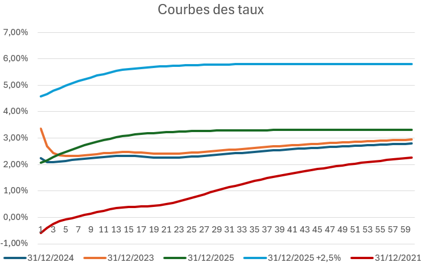
\includegraphics[width=0.9\textwidth]
    {images/2_chapitres/chapitre2/courbe_des_taux_utilisés.png}
    \caption{Courbes de taux retenues pour la construction de la base de données}
    \label{fig:courbes_taux}
\end{figure}

 Ces tableaux permettent de comparer l'impact des différentes sensibilités au 31/12/2025 sur les différentes variables testées.

\begin{figure}[H]
    \centering
    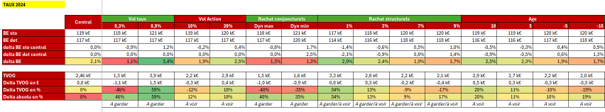
\includegraphics[width=0.95\textwidth]
    {images/2_chapitres/chapitre2/tableau_sensi_2025_1.png}
    \caption{Résultats de l'étude préliminaire de sensibilité -- première partie}
    \label{fig:sensi_1}
\end{figure}

\begin{figure}[H]
    \centering
    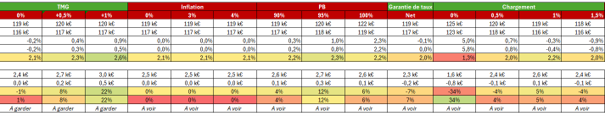
\includegraphics[width=0.95\textwidth]
    {images/2_chapitres/chapitre2/tableau_sensi_2025_2.png}
    \caption{Résultats de l'étude préliminaire de sensibilité -- deuxième partie}
    \label{fig:sensi_2}
\end{figure}

\begin{figure}[H]
    \centering
    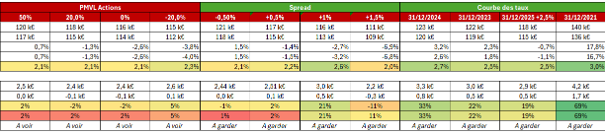
\includegraphics[width=0.95\textwidth]
    {images/2_chapitres/chapitre2/tableau_sensi_2025_3.png}
    \caption{Résultats de l'étude préliminaire de sensibilité -- troisième partie}
    \label{fig:sensi_3}
\end{figure}


\subsection{Construction de la variable de duration}

À la suite des études préliminaires, l'âge des assurés et les rachats structurels n'ont pas été intégrés séparément dans la base de données définitive.

Ces deux variables ont été regroupées à travers une variable de duration du passif. En effet, l'âge des assurés et leur comportement de rachat influencent tous les deux la durée pendant laquelle les contrats restent dans le portefeuille.

La variable de duration permet donc de résumer une partie de l'information portée par ces deux facteurs. Une duration faible correspond à un écoulement plus rapide du passif, tandis qu'une duration élevée correspond à des engagements conservés plus longtemps dans le portefeuille.


\subsection{Sélection des variables définitives}

À la suite des deux études préliminaires, seules les variables ayant l'impact le plus important sur la TVOG ont été conservées.

Les neuf variables retenues sont :

\begin{enumerate}
    \renewcommand{\labelitemi}{\textbullet}
    \item la courbe des taux ;
    \item le spread ;
    \item la volatilité des taux ;
    \item la volatilité des actions ;
    \item la garantie de taux ;
    \item le taux de plus-values latentes sur les actions ;
    \item les rachats conjoncturels ;
    \item la duration du passif ;
    \item le TMG.
\end{enumerate}

Ces variables permettent de représenter à la fois l'environnement économique, les caractéristiques des contrats, la structure du passif et le comportement des assurés.


\subsection{Amplitude des sensibilités retenues}

Pour chacune des variables sélectionnées, plusieurs modalités sont définies autour d'une configuration centrale. 

Les cellules grisées correspondent à la configuration centrale du portefeuille. Cette configuration constitue le point de référence de l'étude. Les autres modalités correspondent à des sensibilités à la hausse ou à la baisse par rapport à cette situation centrale.

\begin{figure}[H]
    \centering
    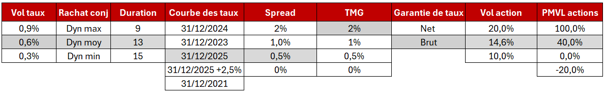
\includegraphics[width=0.95\textwidth]
    {images/2_chapitres/chapitre2/recap_variables.png}
    \caption{Synthèse des variables et des modalités retenues dans la base de données}
    \label{fig:recap_variables}
\end{figure}


\subsection{Taille de la base de données}

La base de données est obtenue en croisant l'ensemble des modalités retenues pour les neuf variables explicatives.

Le nombre total de configurations est donc égal à :

\begin{equation}
    3 \times 3 \times 3 \times 5 \times 4
    \times 4 \times 2 \times 3 \times 4
    = 51\,840.
\end{equation}

La base de données finale contient ainsi \(51\,840\) lignes. Chaque ligne correspond à une configuration particulière du portefeuille et contient :

\begin{itemize}
    \item les valeurs prises par les neuf variables explicatives ;
    \item le Best Estimate déterministe ;
    \item le Best Estimate stochastique ;
    \item l'écart normalisé entre les deux valorisations.
\end{itemize}

La construction de cette base a donc nécessité le lancement de \(51\,840\) projections dans SALLTO.

Le GSE dépend de trois niveaux de volatilité des taux, de trois niveaux de volatilité des actions et de cinq courbes de taux. Il a donc été nécessaire de générer :

\begin{equation}
    3 \times 3 \times 5 = 45
\end{equation}

jeux de scénarios économiques distincts.

Pour chacun de ces jeux de scénarios, les autres variables ont ensuite été combinées directement dans SALLTO afin d'obtenir l'ensemble des \(51\,840\) configurations.


% =============================================================================
% AUTOMATISATION
% =============================================================================

\subsection{Lancement automatisé de SALLTO}

Le lancement manuel de \(51\,840\) projections n'était pas envisageable compte tenu du volume de calculs nécessaire. Une procédure d'automatisation a donc été mise en place afin de lancer successivement les différentes configurations dans SALLTO.

Cette automatisation poursuit plusieurs objectifs :

\begin{itemize}
    \item modifier les hypothèses du fichier d'entrée ;
    \item sélectionner le jeu de scénarios économiques correspondant ;
    \item lancer automatiquement SALLTO ;
    \item attendre la fin de chaque projection ;
    \item récupérer et enregistrer les fichiers de sortie ;
    \item associer chaque résultat à la configuration correspondante ;
    \item regrouper les résultats dans une base de données unique.
\end{itemize}

% À compléter avec la description précise de ton programme :
% - langage utilisé ;
% - utilisation éventuelle de pywinauto ;
% - organisation des boucles ;
% - nommage des outputs ;
% - contrôle de la fin du calcul ;
% - extraction du BE déterministe et du BE stochastique ;
% - temps total de lancement ;
% - gestion des erreurs.